    %LTeX: language=it
\subsection{UC 11 - Modifica cartella} \label{sec:UC11}
\begin{itemize}
    \item \textbf{Attore principale}: MUA;
    \item \textbf{Descrizione}: il MUA deve poter modificare una cartella nel sistema;
    \item \textbf{Precondizioni}: l’account che il MUA gestisce è registrato nel sistema, ha una connessione aperta con il sistema ed è autenticato;
    \item \textbf{Postcondizioni}: la cartella è stata modificata con successo, ed è stata salvata nel sistema;
    \item \textbf{Scenario principale}:
        \begin{enumerate}
            \item il MUA trasmette il nuovo nome della cartella (\hyperref[sec:UC11.1]{UC 11.1});
            \item il MUA trasmette il nuovo id della cartella genitore (\hyperref[sec:UC11.2]{UC 11.2});
            \item il sistema salva la nuova cartella;
        \end{enumerate}
    \item \textbf{Inclusioni}: nessuna;
    \item \textbf{Generalizzazioni}: nessuna;
    \item \textbf{Estensioni}: nessuna.
\end{itemize}

\begin{figure}[H]
    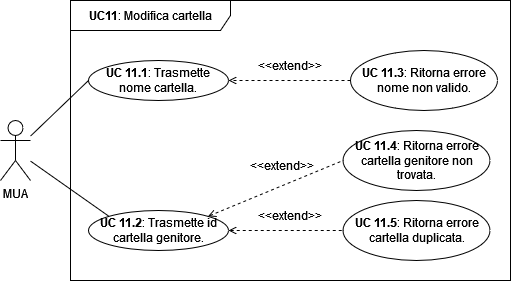
\includegraphics[width=0.85\textwidth]{sections/uc_imgs/UC11.png}
    \centering
    \caption{Diagramma sotto-casi UC 11}
\end{figure}

\subsubsection{UC 11.1 - Trasmette nome cartella} \label{sec:UC11.1}
\begin{itemize}
    \item \textbf{Attore principale}: MUA;
    \item \textbf{Descrizione}: il MUA trasmette il nuovo nome per modificare la cartella al sistema;
    \item \textbf{Precondizioni}: il MUA sta usando la funzionalità di modifica di una cartella;
    \item \textbf{Postcondizioni}: il sistema conosce il nuovo nome della cartella;
    \item \textbf{Scenario principale}:
        \begin{enumerate}
            \item il MUA invia il nuovo nome per modificare la cartella al sistema;
            \item il sistema controlla che le informazioni ricevute rispettino il seguente requisito minimo:
            \begin{itemize}
                \item il nome ricevuto non è una stringa vuota;
            \end{itemize}
        \end{enumerate}
    \item \textbf{Inclusioni}: nessuna;
    \item \textbf{Generalizzazioni}: nessuna;
    \item \textbf{Estensioni}:
        \begin{enumerate}[label=\alph*.]
            \item il sistema non riesce a modificare la cartella perché il nome fornito non è valido:
            \begin{enumerate}[label=\arabic*.]
                \item il sistema ritorna un errore al MUA di nome non valido (\hyperref[sec:UC11.3]{UC 11.3}).
            \end{enumerate}
        \end{enumerate}
\end{itemize}

\subsubsection{UC 11.2 - Trasmette id cartella genitore} \label{sec:UC11.2}
\begin{itemize}
    \item \textbf{Attore principale}: MUA;
    \item \textbf{Descrizione}: il MUA trasmette l'id della nuova cartella genitore al sistema;
    \item \textbf{Precondizioni}: il MUA sta usando la funzionalità di modifica di una cartella;
    \item \textbf{Postcondizioni}: il sistema conosce l'id della nuova cartella genitore;
    \item \textbf{Scenario principale}:
        \begin{enumerate}
            \item il MUA invia l'id della nuova cartella genitore per modificare la cartella;
            \item il sistema elabora le informazioni ricevute, controlla che:
            \begin{itemize}
                \item la cartella genitore esista;
            \end{itemize}
        \end{enumerate}
    \item \textbf{Inclusioni}: nessuna;
    \item \textbf{Generalizzazioni}: nessuna;
    \item \textbf{Estensioni}:
        \begin{enumerate}[label=\alph*.]
            \item il sistema non riesce a salvare la cartella perché non trova la cartella genitore:
            \begin{enumerate}[label=\arabic*.]
                \item il sistema ritorna un errore al MUA di cartella genitore non trovata (\hyperref[sec:UC11.4]{UC 11.4});
            \end{enumerate}
            \item il sistema non riesce a modificare la cartella perché è un duplicato:
            \begin{enumerate}[label=\arabic*.]
                \item il sistema ritorna un errore al MUA di cartella duplicata (\hyperref[sec:UC11.5]{UC 11.5});
            \end{enumerate}
        \end{enumerate}
\end{itemize}



\subsubsection{UC 11.3 - Ritorna errore nome non valido} \label{sec:UC11.3}
\begin{itemize}
    \item \textbf{Attore principale}: MUA;
    \item \textbf{Descrizione}: il MUA riceve l'errore che il nuovo nome della cartella non è valido;
    \item \textbf{Precondizioni}:  il MUA ha trasmesso il nome per modificare la cartella al sistema;
    \item \textbf{Postcondizioni}: il sistema non modifica la cartella e il MUA viene notificato dell'errore;
    \item \textbf{Scenario principale}:
        \begin{enumerate}
            \item il sistema controlla la sintassi del nome e trova un errore;
            \item il sistema non modifica la cartella e notifica il MUA dell'errore;
        \end{enumerate}
    \item \textbf{Inclusioni}: nessuna;
    \item \textbf{Generalizzazioni}: nessuna;
    \item \textbf{Estensioni}: nessuna.
\end{itemize}

\subsubsection{UC 11.4 - Ritorna errore cartella genitore non trovata} \label{sec:UC11.4}
\begin{itemize}
    \item \textbf{Attore principale}: MUA;
    \item \textbf{Descrizione}: il MUA riceve l'errore che la cartella genitore non è stata trovata;
    \item \textbf{Precondizioni}: il MUA ha trasmesso l'id della cartella genitore al sistema;
    \item \textbf{Postcondizioni}: il sistema non modifica la cartella e il MUA viene notificato dell'errore;
    \item \textbf{Scenario principale}:
        \begin{enumerate}
            \item il sistema non trova l'di fornito;
            \item il sistema non modifica la cartella e notifica il MUA dell'errore;
        \end{enumerate}
    \item \textbf{Inclusioni}: nessuna;
    \item \textbf{Generalizzazioni}: nessuna;
    \item \textbf{Estensioni}: nessuna.
\end{itemize}

\subsubsection{UC 11.5 - Ritorna errore cartella duplicata} \label{sec:UC11.5}
\begin{itemize}
    \item \textbf{Attore principale}: MUA;
    \item \textbf{Descrizione}: il MUA riceve l'errore che la cartella è duplicata;
    \item \textbf{Precondizioni}: il MUA ha trasmesso i dettagli per modificare la cartella al sistema;
    \item \textbf{Postcondizioni}: il sistema non modifica la cartella e il MUA viene notificato dell'errore;
    \item \textbf{Scenario principale}:
        \begin{enumerate}
            \item il sistema nota che la cartella esiste già e annulla l'operazione per la modifica della cartella;
            \item il sistema non modifica la cartella e notifica il MUA dell'errore;
        \end{enumerate}
    \item \textbf{Inclusioni}: nessuna;
    \item \textbf{Generalizzazioni}: nessuna;
    \item \textbf{Estensioni}: nessuna.
\end{itemize}

